%\documentclass{article}
%\usepackage{graphicx,subfigure}
%\begin{document}

\begin{figure}[!h]
  \centering
   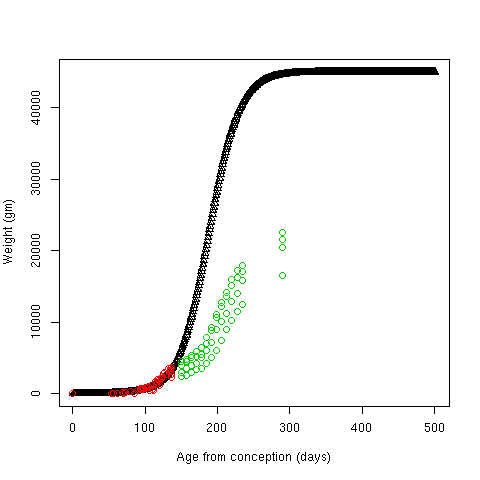
\includegraphics[width=0.9\textwidth]{lwagefit2.png}
%  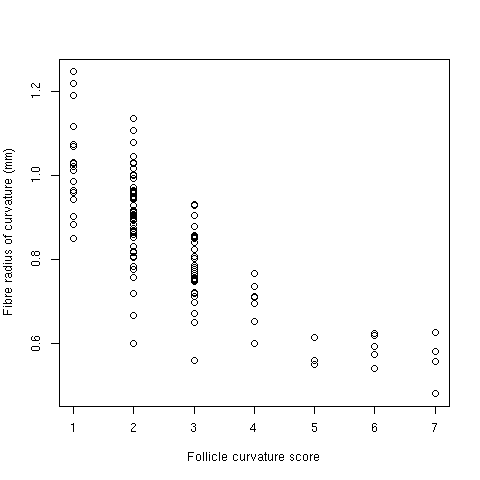
\includegraphics{ofdamm.png}
  \caption{Plot of foetal body weight data from Metcalf etal(1962)~\cite{metc:62} (red circles) with the simulated foetal bodyweights from our generalised logistic equation~\ref{eqn:logi} superimposed (black triangles). Postnatal growth data from Taplin and Everitt(1962)~\cite{tapl:62} are superimposed as green circles.  Parameters for the logistic equation were, $A=0$, $K=45000$, $B=.048$, $\nu=1$, $Q=8000$,$C=1$. Points were calculated over the range zero to 500 days}
  \label{fig:mlbwagefit}
\end{figure}

%\end{document}

